\chapter{\textbf{Literature review}}  \label{chapter:lit}

According to \cite{chowdhury2003} ``Natural Language Processing (NLP) is an area of research and application that explores how computers can be used to understand and manipulate natural language text or speech to do useful things''. In order to build the right tools and techniques to enable computer systems to comprehend and manipulate natural languages to carry out specified tasks, researchers in natural language processing seek to learn about how people interpret and use language.\\

Working with quantitative and qualitative data simultaneously is one of the benefits of using documents, texts, and minutes \cite[p. 1]{bholat2015text}. Even while these types of studies have a wide range of applications, they have only recently been employed in economics despite the fact that working with both types of data makes it possible to conduct research and draw statistical inferences that are not achievable with simply structured data. In this way, it would be possible to have a better understanding of what happens in the economic scenario behind models that we work with NLP -- understanding feelings and emotions of economic agents has always been a goal of science, whether for a better understanding of its uses or even in terms of behavior of the consumer.\\

In a recent study, \cite{shapiro2020measuring} presents new evidence that incorporate NLP techniques into economic science. According to the authors, it was possible to obtain a sentiment index that matched the Michigan Consumer Sentiment Index (MCSI)\footnote{\url{http://www.sca.isr.umich.edu/}}, from economic articles and assessed financials. In terms of methodology, it would then be possible to obtain an index of consumer sentiment through selected journals and textual sentiment analysis techniques. Two studies were proposed: first, it would be analyzed whether the sentiment index elaborated by the authors would be a good predictor variable for real economic variables. For this exercise, the authors used three models of variable selection as a methodological approach: a LASSO, an Adaptive LASSO and a Group LASSO. The variable selection models showed that the sentiment index is significant in the predictor aspect, even when compared to the Michigan Consumer Sentiment Index, the LASSO Group points out the authors' index (based on sentiment techniques) as superior in some models ``Specifically, at least one of the LASSO versions prefers the news sentiment measure in forecasts of employment, output (IP), inflation, the real rate (FFR), and the S\&P 500'' \cite[p. 26]{shapiro2020measuring}. The economic variables used for this study were: employment, output, inflation, the real rate, the consumption, the S\&P 500, the MCSI, and the Conference Board's Consumer Confidence index, in addition to the authors' sentiment index.\\

In a second exercise carried out by the authors, it was analyzed how economic activity would react to a positive shock in the sentiment index. Unlike the conventional method (from an autoregressive vector), the impulse response functions were obtained through local projections \cite{jorda2005estimation} (similar to VAR, but with a less restrictive approach). The results obtained demonstrate that a positive shock in the sentiment index would lead to a slight increase in consumption, in the economy's output, in the real interest rate and in the price level. In addition to these results, impulse responses were also estimated for the Michigan Consumer Sentiment Index and the Conference Board's Consumer Confidence index (CBCI). When analyzing the responses of economic activity to the MCSI, the economic variables (with the exception of the interest rate that responds positively) were not statistically significant. When analyzing the responses of the economic variables to a CBCI choue, the results are similar to the results obtained with the authors' sentiment index -- the responses of the economic variables are statistically significant and point to a slight increase.\\

From economic articles, then, it is possible to analyze and better understand the economic situation. The extraction of a sentiment index through NLP techniques also saves the time and funds needed to obtain an index of this content. With the passage of time, the NLP techniques will evolve, allowing, thus, an improvement in the computational field and in the part of sentiment analysis applied to the economy.\\

In another article, \cite{shapiro2021taking} analyzes Federal Reserve deliberations from NLP techniques to estimate central bank preferences. In other words, it would be possible to estimate the objective function of some generic central bank from its speeches or internal meetings.\\

Based on the estimation of the central bank's loss function, the results showed that the inflation target for the analyzed period (2000-2011) was approximately 1.5\%. With this result, it is possible to perceive that, as everything indicates, the value of the inflation target would be, therefore, significantly below what the surveys of inflation expectations indicated in the period -- for the long term. However, it has been documented \cite[p.32]{shapiro2021taking} that the position of certain members of the Federal Open Market Committee\footnote{Where the speeches come from.} have sometimes stated that an inflation target of 1.5\% seemed consensus at least until 2009 -- after this period, the inflation target value would be 2.0\%.\\

The article also finds that the ``negativity'' of the FOMC is most affected by economic growth and financial conditions. This statement is supported by \cite{walsh2003speed}, which addresses how central banks end up focusing more on economic growth and \cite{coibion2011monetary} which raises this hypothesis based on empirical estimations of the Taylor rule. In a previous work, \cite{thornton2011does} has already pointed out that the FOMC ends up focusing more on the issue of ```growth in output', and not sustainable employment, the unemployment rate, or any concept of slack, as part of their policy directive from 1979 through 2008'' \cite[p.34]{shapiro2021taking}. A question also raised by the article was how financial variables would behave in the face of FOMC speeches. \cite{bernanke2001should} points out that monetary policy should not, for example, respond to a change in asset prices. Having an opinion that supports this study, former Fed Vice President Don Kohn says that the Fed does not respond to asset prices \cite{kohn2006monetary, kohn2009monetary}.\\

On the other hand, a study by \cite{peek2015should} presents financial variables as good predictors of the Fed's interest rate, when these are incorporated into a Taylor rule that takes into account financial instabilities. Finally, \cite{cieslak2021economics} points out that both a stock market crash and a real negative stock market return affect FOMC discourses, and thus become predictive variables of the Fed's interest rate.\\

In another article, to better investigate consumer behavior and sentiment, \cite{barsky2012information} developed two fundamental strategies: the estimation of a new Keynesian DSGE, and the estimation of several VAR models. Through the answer of a question, ``Turning to economic conditions in the country as a whole, do you expect that over the next five years we will have mostly good times, or periods of widespread unemployment and depression, or what?'' \cite[p.1347]{barsky2012information}, the authors created a variable (E5Y) so that this is the percentage of favorable answers to the question minus the percentage of negative answers to the question plus 100. The authors did the same, then, to a horizon of 12 months ahead, and called the variable E12M, in order to better understand how expectations would vary in different future timeframes. Also, they create the expected personal financial (PFE) variable, according to the answer ``Now looking ahead -- do you think that a year from now you (and your family living there) will be better off financially, worse off, or just about the same as now?'' \cite[p.1371]{barsky2012information} and finally create a consumer expectation index (ICE) according to the equation:

\begin{align} \label{eq:ice}
    ICE = \frac{PFE + E12M + E5Y}{4.1134} + 2.0
\end{align}

another index, the consumer sentiment index (ICS) is developed from a variation of the equation (\ref{eq:ice}):

\begin{align} \label{eq:ics}
    ICE = \frac{PFE + E12M + E5Y + DUR + PFP}{6.7558}
\end{align}

where in the equation (\ref{eq:ics}) DUR represents ``wheater or not it is currently a good time to buy `large household items''' \cite[p.1372]{barsky2012information} and PFP is identical `` to PFE, except that PFP respondents to compare their current financial situation relative to one year ago''\cite[p.1372]{barsky2012information}.\\

Based on this interest in a possible sentiment index, the authors estimated VAR models in order to understand how this index would behave if modeled against variables of economic activity. The authors demonstrate from impulse response functions that economic variables such as consumption would have, given a positive shock on the sentiment index, a temporary positive change. The same happens when analyzing the output of the economy.\\

The authors go further and implement a new Keynesian DSGE model incorporating into the model an ``animal spirit'' effect interpreted as ``noise innovations in the signal about productivity growth''\cite[p.1353]{barsky2012information} and trust, represented by E5Y. Assuming that agents observe the technology level from period to period, a noisy signal of the growth rate can be observed:
\begin{align*}
     s_t = g_t + \varepsilon_{s,t}
\end{align*}
where $g$ is an AR(1) stationary process of growth and the shock $\varepsilon_{s,t}$ is interpreted as the animal spirit shock. E5Y in turn is modeled according to the autoregressive process:
\begin{align*}
     E5Y_t = (1 - \rho_e) + \rho_e E5Y_{t-1} + u_t
\end{align*}
where $u_t$ represents the innovation in confidence\footnote{$u_t$ is also modeled as an autoregressive process of order 1. For further explanation, see \cite[p.1354]{barsky2012information}}.\\

The objective of the DSGE estimation was to compare the results of the impulse responses of an anial spirit shock with the results obtained in the VAR models. This ends up having repercussions on another question: ``why are confidence innovations prognostic of future movements in economic activity''\cite[1356]{barsky2012information}? The estimation results corroborate previous studies \cite{rotemberg1997optimization, christiano2005nominal} on the topic.\\

%
%\begin{figure}[!h]
%    \centering
%    \caption{Impulse response of a positive news sentiment shock on economic activity}
%    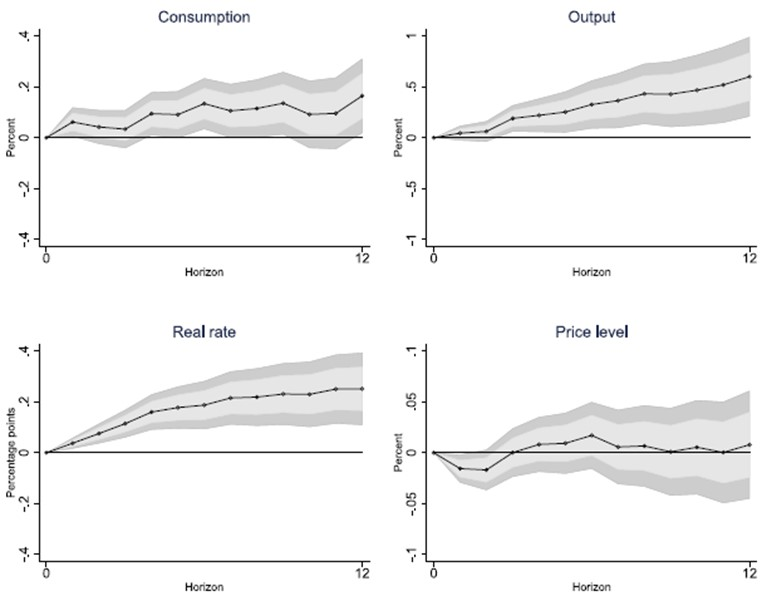
\includegraphics[width=.8\textwidth]{images/image1.jpg}
%    \caption*{Source: \cite[p.16]{shapiro2020measuring}}
%    \label{fig:my_label}
%\end{figure}














In order to complement the literature of sentiment analysis in economics, \cite{ostapenko2020macroeconomic} contributed analysing “how the change of tone or topic in newspaper affects the macroeconomy”. The author transformed articles from newspaper (employing a topic model and vector representation of documents with clustering) into time series and based on this time series, evaluated the sentiment of each article. On occasion, the article demonstrated that given a new shock in the sentiment of the articles, it could mean an increase over the long run, in output and consumption – it also affects the inflation and interest rate, however transiently.\\

Progressively, text mining, sentiment analysis and other techniques end up helping the field of economics to understand better what is happening and what is the relation of the conjunctural or structural scenarios with social expressions. Sentiment analysis helps to understand the consumption behaviour, or even how the media can influence or even chance an economic scenario. Text mining allows to extract qualitative and quantitative information from a text or a corpus. Sooner or later NLP will be increasingly used for a better understanding of the world or the field of economic science.\\

Overall, the approach of researchers and contributors in this area is particularly similar. In terms of estimations, there is a consensus on the importance of treating endogeneity related to macroeconomic relations: when a model is estimated, the use of an autoregressive vector is generally chosen, even if based on an unorthodox approach in the statistical field, considering from methods of Bayesian estimations to autoregressive vector with signal constraints \citet{santos2020indice}.\\

In terms of descriptive analysis, or in terms of classifiers, the approach varies according to the chosen methodology, generally with greater emphasis on classification techniques such as support vector machine, k-means neighbours, or k-nearest neighbour (KNN) \citet{ostapenko2020macroeconomic}. Still, it is worth noting that approaches that assume NLP techniques such as tokenization (see section 3) are still little used, especially with regard to estimations: it is important to emphasize that not using techniques such as tokenization in estimations can create a lack of results in terms of contribution to economic science, given the fact that a better understanding of what happens in the economic scenario is possible and plausible based on a better understanding of how terms and expressions are related to economic cycles.\\



